% Source: graduate-coursework/Sp26/CSCE763/Course_Assignments/HW1/HW1_CSCE_763_solutions.tex

\documentclass[border=4pt]{standalone}
\usepackage{amsmath}
\usepackage{amssymb}
\usepackage{graphicx}
\usepackage{tikz}
\usepackage{xcolor}
\usetikzlibrary{shapes.geometric, arrows.meta, positioning, patterns}

\definecolor{USC_Garnet}{HTML}{73000A}
\definecolor{USC_Sandstorm}{HTML}{FFF2E3}
\definecolor{USC_Black90}{HTML}{363636}
\definecolor{USC_Black70}{HTML}{5C5C5C}
\definecolor{USC_Black50}{HTML}{A2A2A2}
\definecolor{USC_Black10}{HTML}{ECECEC}
\definecolor{USC_Honeycomb}{HTML}{65780B}
\definecolor{USC_Atlantic}{HTML}{466A9F}
\definecolor{USC_Congaree}{HTML}{1F414D}
\definecolor{USC_Rose}{HTML}{CC2E40}
\definecolor{outputbg}{RGB}{245,245,245}

\begin{document}
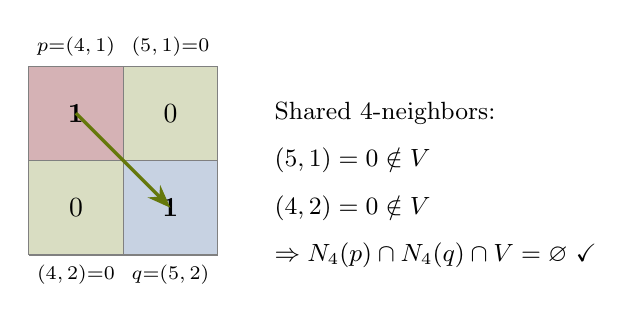
\begin{tikzpicture}[scale=1.2]
    % p
    \fill[USC_Garnet!30] (0,0) rectangle (1,1); \node at (0.5,0.5) {\textbf{1}};
    \node[font=\scriptsize, above] at (0.5,1) {$p{=}(4,1)$};
    % q (diagonal)
    \fill[USC_Atlantic!30] (1,-1) rectangle (2,0); \node at (1.5,-0.5) {\textbf{1}};
    \node[font=\scriptsize, below] at (1.5,-1) {$q{=}(5,2)$};
    % Shared 4-neighbors highlighted
    \fill[USC_Honeycomb!25] (1,0) rectangle (2,1); \node at (1.5,0.5) {0};
    \node[font=\scriptsize, above] at (1.5,1) {$(5,1){=}0$};
    \fill[USC_Honeycomb!25] (0,-1) rectangle (1,0); \node at (0.5,-0.5) {0};
    \node[font=\scriptsize, below] at (0.5,-1) {$(4,2){=}0$};
    % Grid
    \draw[gray, thin] (0,-1) grid (2,1);
    % Diagonal arrow
    \draw[-{Stealth}, very thick, USC_Honeycomb] (0.5,0.5) -- (1.5,-0.5);
    % Labels
    \node[right, font=\small] at (2.5,0.5) {Shared 4-neighbors:};
    \node[right, font=\small] at (2.5,0) {$(5,1) = 0 \notin V$};
    \node[right, font=\small] at (2.5,-0.5) {$(4,2) = 0 \notin V$};
    \node[right, font=\small] at (2.5,-1) {$\Rightarrow N_4(p) \cap N_4(q) \cap V = \varnothing$ \checkmark};
\end{tikzpicture}
\end{document}
